\documentclass[11pt,a4paper]{article}
\PassOptionsToPackage{obeyspaces}{url}
\usepackage[margin=2.1cm]{geometry}
\usepackage{amsmath,amssymb,bm}
\usepackage{graphicx}
\usepackage{booktabs,longtable,array,multirow}
\usepackage[table]{xcolor}
\usepackage{enumitem}
\usepackage{microtype}
\usepackage[colorlinks=true,linkcolor=blue!50!black,citecolor=green!40!black,urlcolor=blue!60!black]{hyperref}
\graphicspath{{../figures_round2/}{../../First round/figures/}}
\setlist{itemsep=1pt,topsep=3pt}
\newcommand{\sq}{\sqrt{f_R}}
\newcommand{\dd}{\mathrm{d}}
\newcommand{\OK}{\textcolor{green!50!black}{\textbf{CONFIRMED}}}
\newcommand{\PART}{\textcolor{orange!85!black}{\textbf{PARTLY}}}
\newcommand{\NO}{\textcolor{red!75!black}{\textbf{INCORRECT}}}
\newcommand{\NV}{\textcolor{gray!80!black}{\textbf{NOT VERIFIABLE}}}
\newcommand{\OVER}{\textcolor{orange!85!black}{\textbf{OVERSTATED}}}
\usepackage{url}
\def\UrlBreaks{\do\/\do\_\do\.\do\-}
\urlstyle{tt}
\newcommand{\file}[1]{{\small\path{#1}}}

\title{Second-round verification of the first agent's work on\\[3pt]
\large ``Gravitational-wave perturbations of a spherical thin shell:\\ junction conditions, scattering coefficients and quasinormal modes''}
\author{Verification report (second round)}
\date{25 September 2026}

\begin{document}
\sloppy
\maketitle

\begin{abstract}
This report documents every check made on the work contained in the folder \file{First round} (the
derivation document \file{derivation/derivation.pdf}, the Python code in \file{code/}, the results in
\file{results/}, the tables and the twelve figures, and the \file{README.md}). For each claim we state how it
was verified -- by re-running the first agent's own code, by an independent re-derivation, by an independent
code written for this purpose, or by reading the cited literature -- and the verdict. The first round is
reproducible bit for bit and its main results for the odd sector and for the static fluid shell (model C) are
confirmed independently, including a new thick-shell derivation of the odd junction condition and a new
Newtonian derivation of the shell's matter modes. We find one substantive physical problem: the
even-parity results of the adiabatically frozen domain wall (model A) are \emph{not} a well-defined
$O(\omega_{\rm dyn}/\omega)$ approximation, but depend at $O(1)$ on which of the Israel equations are imposed.
We also find a number of overstated accuracy claims, catalogue omissions and mislabels, a wrong author name, and
a misprint in the reference paper PSP26. No file of the first round was modified (verified by SHA-256 hashes).
\end{abstract}

\tableofcontents
\newpage

%=====================================================================================================
\section{Scope, material and protocol}\label{sec:protocol}
\paragraph{Material examined.} The task statement \file{PROMPT.md}; the prior notes
\file{Starting point/interior_ondas_cascara.pdf} and \file{burbuja_matching_israel.pdf}; the seven papers of
\file{Bibliography/}; and everything in \file{First round/}: \file{derivation.tex/.pdf} (958 lines), ten
\LaTeX\ tables, the code (\file{main.py}, \file{make_figures.py}, \file{make_tables.py},
\file{polish_catalogue.py}, package \file{shellgw/} with 14 modules, \file{symbolic/} with 5 scripts; the two
auto-generated even-parity junction modules are 1.0 and 1.6 MB of sympy output), the result files
(\file{validation.json}, \file{scattering.json}, \file{qnm_catalogue.json}, \file{qnm_tracks.json},
\file{qnm_table.csv}, 22 log files) and 12 figures (PDF+PNG). All twelve figures were inspected visually.

\paragraph{Non-interference.} Before any action the SHA-256 hash of every file of \file{First round} was stored in
\file{Second round/first_round_sha256_before.txt} (102 files) and compared at the end (Sec.~\ref{sec:integrity}).
The first round's code writes figures and results through relative paths (\file{shellgw/plots.py},
\file{studies.py}); it was therefore \emph{never} executed in place. All executions used copies:
\file{Second round/rerun}, \file{rerun_validate}, \file{rerun_evenC} (execution) and \file{fr_code_pristine}
(read-only import of the generated junction matrices by the independent codes).

\paragraph{Independent material written in the second round} (folder \file{Second round/checks/}; each script
writes an \file{out_*.txt/json} file):
\begin{longtable}{p{6.1cm}p{9.5cm}}
\toprule
script & content\\\midrule
\file{c01_background.py} & symbolic re-derivation of the background Israel equations, I\&S (3.7)--(3.9), static
shell, dust, domain wall, energy/causality bounds, Table~1 numbers.\\
\file{c02_blackhole.py} & own Leaver continued fraction (mpmath, 30 digits); own BH reflectivity (LSODA in $r_*$);
symbolic check of the asymptotic recursion; explicit Iyer--Will 3rd-order WKB formula.\\
\file{c03_axial_thick_shell_derive.py} & from-scratch linearisation of the Einstein equations for axial
perturbations of a static \emph{anisotropic} fluid; master potential.\\
\file{c03b_axial_thick_shell_numeric.py} & smooth thick shell ($p_r=0$) $\to$ thin shell limit of the odd
junction.\\
\file{ind_solver.py} & independent thin-shell solver (mpmath Bessel functions, LSODA, Zerilli asymptotics
without the Chandrasekhar map, different complex ray, secant root finder).\\
\file{c04_compare_scattering_qnm.py} & $\mathcal R,\mathcal T$ and QNMs recomputed and compared with the first
round.\\
\file{c05_newtonian_shell.py} & from-scratch Newtonian theory of the non-radial oscillations of a
self-gravitating fluid shell.\\
\file{c06*_*.py} & properties of the even-parity transfer matrices; model-A prescription dependence.\\
\file{c07_gamma_dependence.py} & $\Gamma$ dependence of the matter modes (vs PSP26 Figs.~1--2).\\
\file{c08_limits.py} & trapped modes, $R\to2M$, low frequency, closed system, NaN point.\\
\file{c09_poles_and_missing_modes.py} & poles of $\mathsf T_{\rm even}$; matter modes missing from the catalogue.\\
\file{integrity_check.sh} & SHA-256 comparison of the first round before/after.\\
\file{make_round2_figures.py} & the five figures of this report.\\\bottomrule
\end{longtable}

\paragraph{Verdict labels.} \OK: verified to the stated accuracy by at least one independent means;
\PART: correct in substance but imprecise, incomplete or only partially checkable; \OVER: numerically true
only in a weaker form; \NO: wrong; \NV: could not be checked with the available sources.

%=====================================================================================================
\section{Summary of findings}\label{sec:summary}
\subsection{Main conclusions}
\begin{enumerate}
\item \textbf{Reproducibility} is complete: re-running the first round's scripts reproduces the symbolic logs,
the whole \file{validation.json} (487 numbers identical to the last bit), all ten \LaTeX\ tables (identical
files) and all twelve figures (pixel-identical).
\item \textbf{Background and choice of model}: all formulas are correct (Sec.~\ref{sec:bg}). The rejection of
``Option B'' (static dust) is correct, but the justification ``the formula $M=4\pi\sigma R^2\sqrt f$ does not follow
from the junction conditions'' is imprecise: that formula \emph{is} the static pressure-balance condition with
$p=0$; it is incompatible with the other junction condition.
\item \textbf{Odd-parity junction} $\Psi_+=\Psi_-$, $\sq\Psi_+'-\Psi_-'=(1-\sq)\Psi/R$ is \OK\ by three independent
routes: (i) a line-by-line re-derivation; (ii) a new derivation of the axial master potential of a smooth
anisotropic fluid, $V=e^{2\Phi}[\ell(\ell+1)/r^2-6m/r^3+4\pi(\rho-p_r)]$, whose thin-shell limit gives exactly
$\Delta_{\rm odd}=4\pi\sigma\sq$; (iii) a numerical thick-shell$\to$thin-shell limit, in which the first round's
junction converges linearly in the thickness while three wrong alternatives do not (Fig.~\ref{fig:thick}).
\item \textbf{Even-parity junction, model C}: \OK. $\det\mathsf T\sq=1$ to $10^{-12}$, $\mathsf T$ real and
flux-conserving for real $\omega$, transparent limit linear in $M$. The matter modes agree with PSP26 Figs.~1--2
(read by us) at all compactnesses and also as functions of $\Gamma$ (a comparison the first round did not make),
and tend to the Newtonian limit that we derived independently (Fig.~\ref{fig:matter}).
\item \textbf{New finding on the reference paper}: PSP26 Eq.~(7.6) contains a misprint (the constant term must be
$-(\ell-1)\ell(\ell+1)[(\ell+2)(2\ell-3)\Gamma-4(\ell-2)]/[16(2\ell+1)]$); their Eq.~(7.8), used by the first
round, is correct.
\item \textbf{Model A (frozen domain wall), even parity}: \NO\ as an approximation with controlled error.
Keeping all four metric-continuity equations, the choice of which two of the four Israel equations are imposed
changes $\mathcal R(\omega)$ by orders of magnitude even at $\omega M=30$ (Fig.~\ref{fig:modelA}), and the lowest
QNMs by 20--30\%. With the first round's choice the energy error $|\mathcal R+\mathcal T-1|$ is \emph{larger than
$\mathcal R$ itself} at all high frequencies, so its $\mathcal R$ has no significant digit. One alternative choice
($\tau\tau$ + trace-free) conserves energy exactly and reproduces the universal $\delta$-barrier law of the odd
sector and of model C. The statement ``the frozen domain wall reflects much more strongly'' is therefore an
artifact of the prescription. Moreover the wall collapses on the light-crossing time
($\omega_{\rm dyn}\simeq\sqrt2/R$), not on $(R^3/M)^{1/2}$ as stated in the Discussion, so the wall's wave QNMs
($|\omega|\approx2$--$5\,\omega_{\rm dyn}$) are not in the adiabatic regime (Fig.~\ref{fig:timescales}).
\item \textbf{Numerics}: $\mathcal R,\mathcal T$ reproduced by an independent solver to $10^{-11}$ (and $\mathcal T$
to $10^{-8}$); every QNM tested reproduced to $10^{-10}$--$10^{-13}$ (damped imaginary matter modes to
$10^{-5}$--$10^{-7}$). The accuracy claims ``QNMs agree to $\lesssim10^{-8}$'' (README) and ``$10^{-8}$--$10^{-13}$''
(derivation) are \OVER: 28 of 397 catalogue modes differ by more than $10^{-8}$ between the two methods, the worst
by $6.4\times10^{-5}$ (still within the required $10^{-4}$).
\item \textbf{Catalogue}: incomplete for compact shells -- the stable matter pair is missing for $\ell=2$ at
$R=2.2,2.5,3M$ (it exists: e.g.\ $0.197121-0.000310i$ at $R=3M$) and the unstable $\ell=4$ mode is missing at $R=2.2M$
($0.43726i$); two modes are mislabelled.
\item \textbf{Literature}: all citations checked exist and are used correctly, except the author of the eikonal
instability paper (Yang, Bonga and \emph{Z.~Pan}, PRL 130, 011402 (2023), not ``U.-L.~Pen'').
\end{enumerate}

\subsection{Claim-by-claim table}
{\small
\begin{longtable}{p{0.6cm}p{7.3cm}p{4.2cm}p{2.7cm}}
\toprule
ID & claim of the first round & how checked & verdict\\\midrule\endhead
\multicolumn{4}{l}{\emph{Reproducibility}}\\
R1 & symbolic scripts reproduce the logs & re-run in copy & \OK\\
R2 & \file{validation.json}, tables, figures follow from the code & re-run, diff, pixel compare & \OK\\
R3 & generated junction modules follow from \file{derive_junction.py} & re-run (Sec.~\ref{sec:repro}) & \OK\\
\multicolumn{4}{l}{\emph{Background (derivation Sec.~1)}}\\
B1 & $\sigma=(1-\sq)/4\pi R$, $p=(1-M/R-\sq)/(8\pi R\sq)$ (P04 3.80--3.81) & sympy (c01) + P04 text & \OK\\
B2 & Israel $\Leftrightarrow$ I\&S (3.7a,b); mass formula (3.8), (3.9) & sympy (c01); IS84 page image & \OK\\
B3 & static shell needs $\tau/\sigma=-\kappa$, $\kappa=(1-\sq)/4\sq$ & sympy & \OK\\
B4 & DEC $\Leftrightarrow R\ge25M/12$; $\Gamma=2$ causality $\Leftrightarrow$ same bound & sympy & \OK\\
B5 & no static dust shell & sympy & \OK\\
B6 & ``$M=4\pi\sigma R^2\sq$ does not follow from the junction conditions'' & sympy & \PART\\
B7 & dust turning point: same geometry, $\ddot R=-M/[R^2(1+\sq)]$ & sympy & \OK\\
B8 & wall: $\ddot R=-M/[R^2(1+\sq)]-2\sq/R=-(1+3\sq)/(2R)$ & sympy; also first-round log & \OK\\
B9 & Table 1 (background.tex) numbers & recomputed & \OK\\
B10 & I\&S quote ``$\ddot R$ always negative if $\tau\ge0$'' & IS84 p.~714 & \OK\\
B11 & interior frequency $\nu=\omega/\sq$ (correction of prompt and prior notes) & P04 (3.75); PSP26 & \OK\\
B12 & ``every thin shell of this type evolves on $(R^3/M)^{1/2}$''; ``growth time comparable to wall collapse'' & Table 1, c01 & \NO\\
\multicolumn{4}{l}{\emph{Perturbation equations (Sec.~2--3)}}\\
P1 & $V_{\rm Z}$ (Zerilli Eq.~5) $=f\times$MP05 (4.26) & re-run (residual 0) & \OK\\
P2 & odd reconstruction $h_t=\tfrac f2(r\Psi)'$, $h_r=-i\omega r\Psi/2f$ & re-run (5 residuals 0); MP05 (5.18) & \OK\\
P3 & even reconstruction Eqs.~(2.8)--(2.10), $Q(r)$ & re-run + sympy comparison with the printed formulas & \OK\\
P4 & first-order system agrees with Zerilli (1970) & compared with Z70 p.~737 & \OK\\
P5 & Chandrasekhar map, amplitude factor $\mu(\mu+2)+12iM\omega$ & re-run; analytic & \OK\\
P6 & Riccati--Bessel/Hankel functions, Wronskian $=1$ & mpmath (ind\_solver) & \OK\\
\multicolumn{4}{l}{\emph{Odd junction (Sec.~4.2)}}\\
O1 & $\delta K_{tA}$, $\delta K_{AB}$ (Eq.~4.4) & hand re-derivation & \OK\\
O2 & $AB$ equation $\Rightarrow\Psi_+=\Psi_-$; $\tau A$ $\Rightarrow U=0$; $[K]^{(0)}$ and $p$ cancel & hand & \OK\\
O3 & final junction (4.8), $\Delta_{\rm odd}=\sq(1-\sq)/R$, $\det\mathsf T=f^{-1/2}$ & thick-shell theory + numerics (c03) & \OK\\
O4 & agreement with PSP26 (5.23) and Pani et al.\ (3.29), (A35) & read both papers & \OK\\
O5 & model-A odd system consistent (rank 3) & first-round log & \OK\\
\multicolumn{4}{l}{\emph{Even junction (Sec.~4.3)}}\\
E1 & $\det\mathsf T^{\rm C}=f_R^{-1/2}$ ($10^{-12}$ double, $10^{-15}$ mp) & 300 random samples (c06) & \OK\\
E2 & flux conservation, $\mathcal R+\mathcal T=1$ & $\mathsf T$ real, flux $10^{-13}$ (c06) & \OK\\
E3 & transparent limit $4\times10^{-9}$ at $M=10^{-8}$ & c06 & \OK\\
E4 & double precision error $10^{-6}$ at $R=2.2M$, breakdown $R\lesssim2.05M$ & c06: $1.3\times10^{-7}$; $5\times10^{-3}$ at 2.05 & \PART\\
E5 & $\mathsf T$ has poles at the matter-mode frequencies & zeros of $\det\mathsf A$ (c09) & \PART\\
E6 & matter modes reproduce PSP26 Figs.~1--2 and PN limit Eq.~(7.8) & PSP26 read; own solver; own Newtonian theory & \OK\\
E7 & wave modes agree with PSP26 Figs.~3--4 to $\pm0.02$ & PSP26 read & \OK\\
E8 & even-C merges with odd at high frequency ($\delta$-barrier law) & own solver (c06c) & \OK\\
\multicolumn{4}{l}{\emph{Model A (Sec.~4.3, 6)}}\\
A1 & rank$\,\mathsf A=6$, rank$[\mathsf A|\mathsf B]=8$ & first-round log & \OK\\
A2 & constraints violated $\propto\omega^{-1}$, $|\mathcal R+\mathcal T-1|\propto\omega^{-2}$ & c06 (exponent $-2.00$) & \OK\\
A3 & $\dddot T_0\propto\ddot R^2\neq0$ at the turning point & analytic & \OK\\
A4 & even-A results ``$O(\omega_{\rm dyn}/\omega)$-accurate'' & six prescriptions (c06d, c06e) & \NO\\
A5 & ``frozen domain wall reflects much more strongly'' & same & \NO\\
\multicolumn{4}{l}{\emph{Numerics (Sec.~5--6)}}\\
N1 & continued fraction (Pani B4 with $\omega\to-\omega$), convergence iff $R_2\ge4M$ & re-run; Pani App.~B & \OK\\
N2 & asymptotic recursion Eq.~(5.5) & sympy (c02) & \OK\\
N3 & M1 vs M2 on $\mathcal R$, $\mathcal T$: $\lesssim10^{-10}$ & table: $6\times10^{-10}$; own solver & \PART\\
N4 & M1 vs M2 on QNMs: $10^{-8}$--$10^{-13}$ / README $\lesssim10^{-8}$ & catalogue: max $6.4\times10^{-5}$ & \OVER\\
N5 & QNM values & own solver, $10^{-10}$--$10^{-13}$ & \OK\\
N6 & catalogue/tables list the lowest modes & own searches & \PART\\
N7 & Boyanov et al.\ estimator implemented, agrees within $O(1/r)$ & table (2--4$\times10^{-6}$) & \OK\\
N8 & NaN at $\ell=4$, $\omega M=0.0057$ & \file{scattering.json} & \OK\\
\multicolumn{4}{l}{\emph{Schwarzschild validation and limits}}\\
S1 & $\ell=2,n=0$: $0.37367168-0.08896232i$ & own Leaver (30 digits) & \OK\\
S2 & $n\le3$, $\ell=2,3,4$ agree with BCS09 to 6 digits & own Leaver vs 6-digit table & \OK\\
S3 & WKB orders 1, 3, 6; IW Table~I values & explicit IW formula (order 3) & \OK\ (3) / \NV\ (6)\\
S4 & quoted WKB errors $7\times10^{-2}$, $1.5\times10^{-3}$, $2.3\times10^{-4}$ & recomputed: these are \emph{relative} errors & \PART\\
S5 & BH reflectivity $1.55\times10^{-2}$, $5.3\times10^{-9}$; Vishveshwara Fig.~2 & own integrator; V70 scan & \OK\\
L1 & low frequency: $1-\mathcal R<10^{-11}$ & own solver: $10^{-15}$ & \OK\\
L2 & high frequency: $\mathcal R\simeq\Delta^2/4\omega^2$ (odd) & own solver: ratio $\to1$ & \OK\\
L3 & $\mathcal R\to\mathcal R_{\rm BH}$ as $R\to2M$ & own solver down to $R=2.0002M$ & \PART\\
L4 & closed system $|S|=1$ & own solver: $10^{-16}$ & \OK\\
L5 & trapped modes; WKB Re to 1--6\%, Im within factor $\lesssim2$ & own solver ($10^{-12}$); 0.6--6.3\%, up to 2.03 & \PART\\
\multicolumn{4}{l}{\emph{Literature and task compliance}}\\
C1 & PSP26 exists, same system, equation numbers and content & PDF read & \OK\\
C2 & Boyanov et al., PRL 135, 151402 (2025) & INSPIRE & \OK\\
C3 & other citations (Tab.~\ref{tab:lit}) & INSPIRE/ADS/local PDFs & \OK\ except one\\
C4 & ``H.~Yang, B.~Bonga and U.-L.~Pen'' & APS/INSPIRE & \NO\\
C5 & every function has a docstring citing an equation & AST audit & \PART\\
C6 & required plots, CSV columns, tolerances & inspection & \OK\\\bottomrule
\end{longtable}}

%=====================================================================================================
\section{Reproducibility}\label{sec:repro}
\paragraph{Symbolic scripts.} In the copy \file{Second round/rerun} we executed
\file{symbolic/vacuum_relations.py} (33\,s) and \file{symbolic/exterior_series.py} (1.5\,s). The outputs
(\file{rerun/rerun_log_vacuum.txt}, \file{rerun_log_exterior_series.txt}) coincide with the first-round logs
\file{log_vacuum_relations.txt} and \file{log_exterior_series.txt}: the Zerilli/MP05 potential identity, the five
odd vacuum residuals, the CPM reconstruction, the even first-order system, the algebraic identity, the
reconstruction formulas and the ``max residual of all 6 vacuum Einstein equations \dots = 0'' are all
reproduced, as is the $c,d,e$ polynomial check and the Chandrasekhar-map residual $0$.
\file{derive_junction.py} was re-run for all four cases (\file{rerun/}) and separately for the even model-C
case (\file{rerun_evenC/}); see the note at the end of this section for its outcome.

\paragraph{Numerical stage.} \file{main.py validate} was executed in \file{rerun_validate} (38\,s). The new
\file{validation.json} was compared recursively with the original: all 487 numbers are identical to the last bit.
\file{make_tables.py} regenerates the ten tables of the derivation: all ten files are byte-identical.
\file{make_figures.py} regenerates the twelve figures from the stored results: all PNGs are pixel-identical.
The long stages (\file{scatter}, 546\,s, and \file{qnm}, 3283\,s, on 10 cores) were not re-run as a whole;
instead their outputs were \emph{recomputed with independent code} (Secs.~\ref{sec:num}), which is a stronger test.

\paragraph{Junction-module regeneration.} \file{derive_junction.py} was re-run in fresh copies. For the even sector (\file{even:C}, 32\,s;
\file{even:A}, 43\,s) the log lines of the first round are reproduced verbatim (background residual 0, $\ddot R$ for the
wall, ranks $8/8$ and $6/8$, residual $4.62\times10^{-15}$ and $7.12\times10^{-3}$, the test matrices $\mathsf T$), the
pickled symbolic matrices $\mathsf A,\mathsf B$ (and $\ddot R$) are \emph{structurally identical} to the first round's,
and the exported Python modules are identical apart from the UTF-8 byte-order mark and the final line ending. For the
odd sector the full script did not finish within 35 minutes: after exporting the matrices it attempts an optional
symbolic \texttt{sympy.solve}/\texttt{simplify} of the system (whose output is only printed; the first-round log also
stops before that line). Calling the script's \texttt{derive()} function directly, the odd $\mathsf A,\mathsf B$ of models C
and A are obtained in 1\,s; they differ from the stored ones only in the printed form of the expressions and agree
numerically to $1.5\times10^{-13}$ (the resulting $\mathsf T$ to $3\times10^{-15}$) at random complex parameters. Hence
all four generated junction systems are reproducible (R3 \OK).


%=====================================================================================================
\section{Background spacetime, collapse problem and choice of model}\label{sec:bg}
\paragraph{Method.} In \file{c01_background.py} the jumps of the mixed extrinsic curvature,
$K^\theta{}_\theta|_\pm=\{\beta,\alpha\}/R$, $K^\tau{}_\tau|_+=(\ddot R+M/R^2)/\beta$, $K^\tau{}_\tau|_-=\ddot R/\alpha$
[IS84 (3.5)--(3.6), whose page we rendered and read], were inserted into
$[K^a{}_b]-\delta^a_b[K]=-8\pi S^a{}_b$ with $S^a{}_b={\rm diag}(-\sigma,p,p)$ and solved for $\sigma,p$.

\paragraph{Results.}
\begin{itemize}
\item I\&S (3.7a) and (3.7b) (with $\tau=-p$) are satisfied identically by these $\sigma,p$ (numerical residuals
$5\times10^{-17}$ and $0$ at a random point with $\dot R\ne0$); the mass formula (3.8) holds to $10^{-16}$; at
$\dot R=0$, $4\pi\sigma R=1-\sq$ and (3.9) holds exactly (B2 \OK).
\item Static shell: $\sigma=(1-s)/4\pi R$, $p=(1-s)^2/(16\pi Rs)$ with $s=\sq$; this equals Poisson's (3.81)
(residual 0) and $\kappa=p/\sigma=(1-s)/4s=M/[2Rs(1+s)]$ (B1, B3 \OK).
\item $\kappa=1$ and $v_s^2=2\kappa/(1+\kappa)=1$ both occur at $s=1/5$, i.e.\ $R=25M/12$ (B4 \OK).
\item Dust: $p=0$ with $\dot R=\ddot R=0$ forces $s=1$ ($M=0$) (B5 \OK). At a turning point
$\ddot R=-(1-s)/2R=-M/[R^2(1+s)]$ (B7 \OK).
\item Domain wall ($p=-\sigma$) at $\dot R=0$: $\ddot R=-(1+3s)/2R$, equal to $-M/[R^2(1+s)]-2s/R$ (B8 \OK).
All nine columns of Table~1 (\file{background.tex}) are reproduced to all printed digits (B9 \OK).
\end{itemize}
\paragraph{Remark on Option B (B6, \PART).} For a static shell the pressure equation
$8\pi p=[K^\tau{}_\tau]+[K^\theta{}_\theta]$ with $p=0$ gives $[K^\tau{}_\tau]=M/(R^2\sq)=4\pi\sigma$, i.e.\ exactly the
task's formula $M=4\pi\sigma R^2\sq$. So that formula \emph{does} follow from one junction condition; it is the
second one, $4\pi\sigma R=1-\sq$, that is incompatible with it unless $M=0$. The first round's conclusion is right,
its wording is not.

\paragraph{Time scales (B12, \NO).} The Discussion states that ``every thin shell of this type evolves on the
timescale $(R^3/M)^{1/2}$'' and that the model-C growth time $\sim1.6(R^3/M)^{1/2}$ ``is comparable to the collapse
time of the domain wall''. From $\ddot R=-(1+3\sq)/2R$ one has $\omega_{\rm dyn}=\sq(|\ddot R|/R)^{1/2}\to\sqrt2/R$
for $R\gg M$: a tension-dominated wall collapses on the light-crossing time, independently of $M$. At $R=6M$
the wall's collapse time is $1/\omega_{\rm dyn}=5.6M$ while the model-C growth time is $1/0.0401=25M$; at $R=10M$,
$8.2M$ vs $57M$. Fig.~\ref{fig:timescales} shows that $\omega_{\rm dyn}$ is of the same order as the wave-mode
frequencies, so the argument ``wave-mode QNMs have $\omega\sim1/R\gg(M/R^3)^{1/2}$'' covers model C but not model A.

\begin{figure}[t]\centering
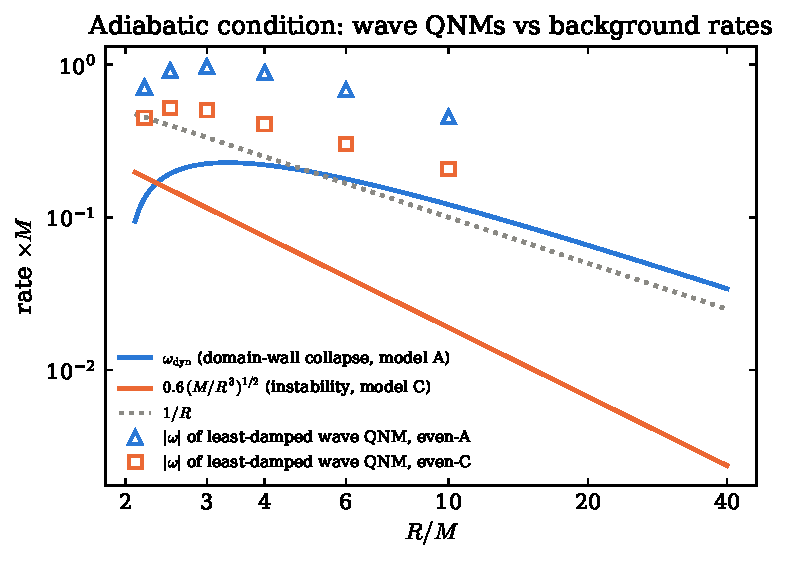
\includegraphics[width=0.62\textwidth]{r2_fig4_timescales.pdf}
\caption{Background rates versus the least-damped wave QNMs ($\ell=2$). The domain-wall collapse rate
$\omega_{\rm dyn}$ follows $\sim1/R$ and is only a factor 2--5 below the model-A wave QNMs, whereas the model-C
instability rate $\propto(M/R^3)^{1/2}$ is well separated.}\label{fig:timescales}
\end{figure}

\paragraph{Blueshift (B11, \OK).} Continuity of $h_{ab}$ at a static shell gives $\dd T=\sq\,\dd t$ (Poisson's
interior metric (3.75), which we read); PSP26 use $w=F^{-1/2}\omega$ inside. The correction to the task statement
and to \file{interior_ondas_cascara} (which uses $\hat\jmath_\ell(\omega r)$) is justified.

%=====================================================================================================
\section{Perturbation equations and interior solution}
The re-run of \file{vacuum_relations.py} gives zero residuals for all statements of derivation Sec.~2 (P1, P2).
We checked that the \emph{printed} reconstruction formulas (2.8)--(2.10), including the polynomial $Q(r)$, are
algebraically identical to the expressions printed in the log (difference simplified to $0$ with sympy) (P3). The
$K'$ equation of the first-round first-order system coincides term by term with Zerilli's (1970, p.~737) system
for $e^{-i\omega t}$ (P4). The Chandrasekhar map is verified by the re-run (residual 0) and for outgoing waves
$Z\to[\mu(\mu+2)+12iM\omega]e^{i\omega r_*}$ follows from $\dd\Psi/\dd r_*=i\omega\Psi$ (P5). Using mpmath
Bessel functions and the exact recurrence $(z j_\ell)'=zj_{\ell-1}-\ell j_\ell$ we verified the Wronskian
$\hat\jmath\hat y'-\hat\jmath'\hat y=1$ (to $10^{-16}$ at real and complex argument) and agreement with
\file{scipy.special} to $10^{-15}$ (P6).

%=====================================================================================================
\section{Odd-parity junction condition}\label{sec:odd}
\subsection{Line-by-line re-derivation}
We re-derived by hand the chain of derivation Sec.~4.2: (a) the covariant form of
$\delta\Gamma^r{}_{t\phi}=\tfrac f2(\partial_th_r-\partial_rh_t)X_\phi$ (the $\Gamma$-terms of the three covariant
derivatives cancel pairwise) and $\delta\Gamma^r{}_{AB}=fh_rX_{AB}$ (using $D_AX_B+D_BX_A=2X_{AB}$); with $n_r=f^{-1/2}$
unperturbed this gives Eq.~(4.4). (b) With the CPM definition $\partial_rh_t-\partial_th_r=\mu\Psi/2r+2h_t/r$, the
proper-time components (4.5) follow. (c) $\delta S_{AB}=0$ gives $[\sq h_r]=0$, and with
$h_r^+=-i\omega R\Psi_+/2f$, $h_r^-=-i\nu R\Psi_-/2$, $\nu=\omega/\sq$, one gets $\Psi_+=\Psi_-$ exactly (for
$\omega\ne0$). (d) In the $\tau A$ equation the combination $[K]^{(0)}\mathcal H-8\pi p\mathcal H=-4\pi\sigma\mathcal H$
is independent of $p$ (hence of $\ddot R$), and $(\sq-1)/R=-4\pi\sigma$ cancels it: $U=0$. (e) Continuity of
$\mathcal H=\tfrac12(r\Psi_-)'=\tfrac{\sq}{2}(r\Psi_+)'$ gives (4.8). All steps are correct (O1, O2 \OK).

\subsection{Independent derivation: axial perturbations of an anisotropic fluid}
Because (a)--(e) share the first round's framework, we derived the odd junction a second time in a completely
different way. In \file{c03_axial_thick_shell_derive.py} we linearised the Einstein equations (own code) for the
static metric $-e^{2\Phi}\dd t^2+\dd r^2/(1-2m/r)+r^2\dd\Omega^2$ with an anisotropic fluid
$T_{\mu\nu}=(\rho+p_t)u_\mu u_\nu+p_tg_{\mu\nu}+(p_r-p_t)s_\mu s_\nu$ ($s$ normal to the matter layers) and an axial
perturbation (metric $h_0,h_1$ and fluid velocity $U$). Eliminating $h_0$ with the $\theta\phi$ equation, the
$r\phi$ equation becomes, for $X=e^{\Phi-\Lambda}h_1/r$ and $\dd r_*=e^{\Lambda-\Phi}\dd r$,
\begin{equation}
\frac{\dd^2X}{\dd r_*^2}+\left[\omega^2-V\right]X=0,\qquad V=e^{2\Phi}\left[\frac{\ell(\ell+1)}{r^2}-\frac{6m}{r^3}+4\pi(\rho-p_r)\right],
\end{equation}
after using $m'=4\pi r^2\rho$, $\Phi'=(m+4\pi r^3p_r)/r(r-2m)$ and the anisotropic TOV equation (sympy: difference 0).
The tangential pressure and the fluid velocity drop out, which is the thick-matter analogue of the first round's
statement that the odd junction is independent of the equation of state. For a shell ($p_r=0$), the
anisotropic TOV equation gives $p_t=\rho r\Phi'/2$, and integrating over the layer gives, as the thickness tends to
zero, surface density $\int\rho\,\dd\ell=(1-\sq)/4\pi R=\sigma$ and surface pressure
$\int p_t\,\dd\ell=(1-\sq)^2/(16\pi R\sq)=p$: exactly model C. The potential contains
$\int4\pi\rho e^{2\Phi}\dd r_*=\sq\,4\pi\sigma$, i.e.\ a $\delta$-function of strength $\Delta_{\rm odd}=4\pi\sigma\sq$,
while the other terms stay bounded. Since $X=(\omega/2i)\Psi_{\rm CPM}$ on both sides (with the interior normalised to
its own time), this reproduces Eqs.~(4.8)--(4.9) exactly.

\subsection{Numerical thick-shell limit}
In \file{c03b} a smooth shell of half-thickness $\varepsilon$ ($\rho\propto[1-(r-R)^2/\varepsilon^2]^2$) was built
numerically, $X$ was integrated from the flat interior through the matter, and the direction of $(X,X')$ at
$r=R+\varepsilon$ was compared with the thin-shell prediction built from the first round's matrix
$\mathsf T_{\rm odd}$ and from three wrong alternatives. Fig.~\ref{fig:thick}: only the first round's matrix gives a
mismatch that tends to zero, linearly in $\varepsilon$ ($6.6\times10^{-4}$ at $\varepsilon=0.006M$, $\omega M=0.2$),
while the alternatives saturate at $4$--$10\times10^{-2}$ (O3 \OK).

\begin{figure}[t]\centering
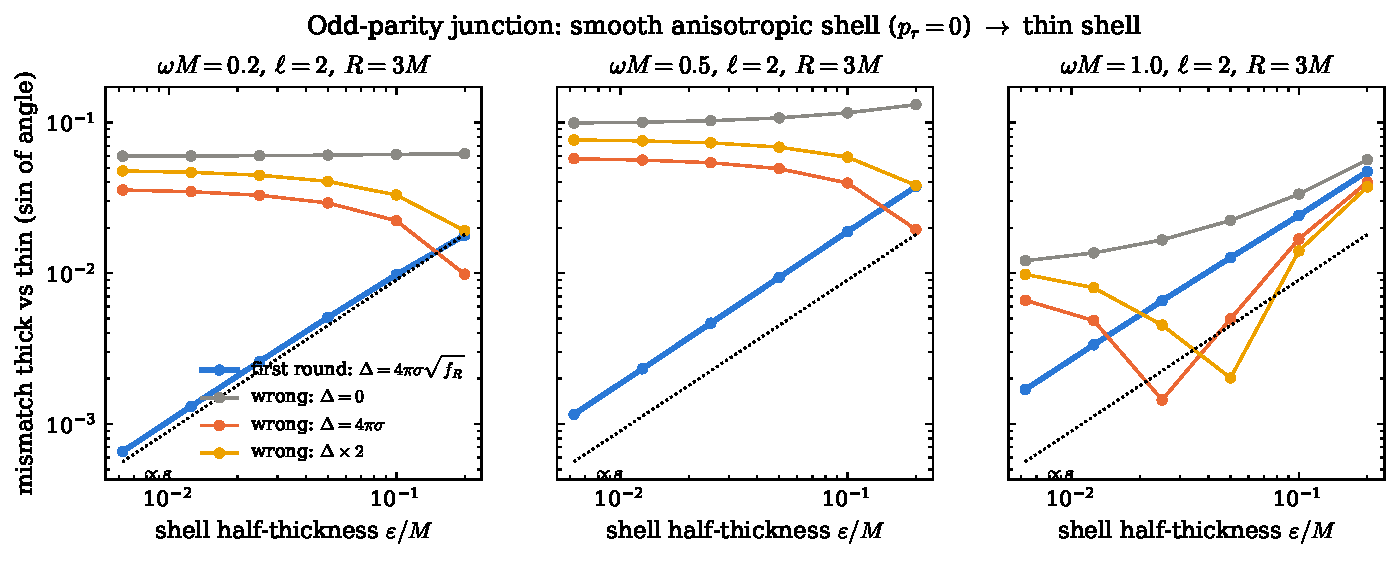
\includegraphics[width=\textwidth]{r2_fig1_thick_shell_limit.pdf}
\caption{Independent test of the odd junction: smooth anisotropic shells of decreasing thickness converge to the
first round's thin-shell junction and to none of the alternatives.}\label{fig:thick}
\end{figure}

\subsection{Literature}
PSP26 Eq.~(5.23), $F^{1/2}\eta_{\rm out}-\eta_{\rm in}+F^{1/2}-1=0$, is on p.~20 of the PDF (we read it). With
$\eta=R\hat\psi'/\hat\psi$ of the retarded-time functions $\hat\psi_{\rm out}=e^{-i\omega r_*}\Psi$ and
$\hat\psi_{\rm in}=e^{-iwr}\Psi$, the extra terms are $F^{1/2}(-i\omega R/F)-(-iwR)=0$ because $w=F^{-1/2}\omega$;
(5.23) is then identical to (4.8). Pani et al.\ (3.29) and (A35) are $[[h_0]]=0$ and $[[\sqrt h\,h_1]]=0$ (read in the
arXiv v2 PDF), and their text states that for continuous $h$ these imply continuity of $\Psi$, $\Psi'$ (O4 \OK).

%=====================================================================================================
\section{Even-parity junction, model C}\label{sec:even}
The even derivation (a symbolic brute-force computation of $\sim2.5$\,MB of expressions) was not repeated
independently. It was tested through its consequences, which is sufficient to validate it within the precision
of the tests.
\begin{itemize}
\item \textbf{Determinant, reality, flux} (\file{c06}). Over 300 random $(\omega,\ell,R,v_s^2)$ with $R\in[2.35,30]M$:
$\max|\det\mathsf T\sq-1|=1.1\times10^{-12}$ (real $\omega$) and $9.2\times10^{-13}$ (complex $\omega$); ${\rm Im}\,\mathsf T=0$
exactly for real $\omega$; the flux $J={\rm Im}(\Psi^*\partial_x\Psi)$ is conserved to $1.6\times10^{-13}$ for arbitrary
interior data (E1, E2 \OK).
\item \textbf{Transparent limit}: $|\mathsf T^{\rm C}-\mathbb I|=4.0\times10^{-5},4.0\times10^{-7},4.0\times10^{-9}$ at
$M=10^{-4},10^{-6},10^{-8}$ (E3 \OK).
\item \textbf{Precision near $2M$} (E4 \PART): in double precision $|\det\mathsf T\sq-1|=10^{-9}$ ($2.3M$),
$1.3\times10^{-7}$ ($2.2M$, the text says $10^{-6}$), $1.6\times10^{-5}$ ($2.1M$), $5\times10^{-3}$ ($2.05M$), $0.87$
($2.02M$); the 40-digit path gives $\le3\times10^{-15}$ down to $2.01M$, as claimed.
\item \textbf{Poles} (E5 \PART): the zeros of $\det\mathsf A(\omega)$ (poles of $\mathsf T$) lie at
$\omega(R^3/M)^{1/2}\approx1.54$ and $0.985i$ ($R=6M$) -- at the matter scale, but not at the matter QNM frequencies
($1.315$, $0.590i$); ``poles at the frequencies of the matter modes'' is loose.
\item \textbf{PSP26 matter modes} (E6 \OK). Reading PSP26 Figs.~1--2 (p.~3--4) we find, for $M/R=0.3\dots0.01$,
${\rm Im}\,\omega(R^3/M)^{1/2}\approx0.668,0.637,0.608,0.582,0.557,0.535,0.518$ and ${\rm Re}\approx
1.096,1.188,1.267,1.336,1.398,1.454,1.495$, ${\rm Im}\approx-1.70,-1.51,-1.10,-0.65,-0.28\,(\times10^{-3})$: the
first round's table agrees at the reading precision ($\pm0.002$). Our independent solver reproduces every entry of
that table to $\le2\times10^{-11}$. Beyond the first round, we compared the $\Gamma$ dependence at $M/R=0.2$
(PSP26 Figs.~1--2, right/lower panels): at $\Gamma=1.81$ and $2.46$ we obtain $0.6437i$, $1.1383-8.2\times10^{-4}i$ and
$0.5511i$, $1.5486-1.93\times10^{-3}i$, against the plotted $0.643$, $1.14$, $-0.82\times10^{-3}$ and $0.551$, $1.548$,
$-1.93\times10^{-3}$.
\item \textbf{Newtonian limit, independent derivation} (\file{c05}). We solved from scratch the Newtonian problem
of a self-gravitating 2D fluid shell (continuity, Laplace-type normal force $2Hp$, self-gravity including the
multipole shift of the displaced mass sheet, $\delta p=\Gamma p\,\delta\sigma/\sigma$). The $2\times2$ eigenproblem
for $\varsigma^2=\omega^2R^3/M$ has trace $[(\ell^2+\ell+4)\Gamma-(\ell^2+\ell+6)]/4$ and determinant
$-(\ell-1)\ell(\ell+1)[(\ell+2)(2\ell-3)\Gamma-4(\ell-2)]/[16(2\ell+1)]$; its roots coincide identically (sympy) with
PSP26 Eq.~(7.8) for all $\ell,\Gamma$. For $\ell=2$, $\Gamma=2$: $\varsigma=1.504962$ and $0.514695i$. The first round's
full-GR values at $M/R=0.01,0.02$ extrapolate (Richardson) to $0.51463i$ and $1.50514$, i.e.\ to this limit.
\item \textbf{Misprint in PSP26}: the quartic (7.6) printed in PSP26 has constant term
$-(\ell-1)\ell(\ell+1)(\ell+2)[(2\ell-3)\Gamma-4]/[16(2\ell+1)]$, which is inconsistent with its own solution (7.8) and
with its Newtonian Eq.~(10.62); for $\ell=2,\Gamma=2$ it would give no unstable mode. The correct constant is the
determinant above. The first round used (7.8) and is unaffected.
\item \textbf{Wave modes} (E7 \OK): the five entries of \file{psp_wave.tex} agree with our reading of PSP26 Figs.~3--4
(e.g.\ odd, $M/R=1/6$, mode 2: ${\rm Re}(R\omega)\approx4.15$, ${\rm Im}(R\omega)/\xi\approx-0.83$). PSP26's
Newtonian formulas (7.23)--(7.25) are quoted correctly.
\item \textbf{High frequency} (E8 \OK). Although $\mathsf T^{\rm C}_{21}$ does not tend to the odd value (the ratio of
the implied $\delta$ strengths is $0.455$, $0.890$, $1.105$ at $R=3,6,10M$), the $O(1/\omega)$ off-diagonal terms
compensate, and the reflectivities do merge: $\mathcal R_{\rm even}/\mathcal R_{\rm odd}=1.0097,1.0002,1.0000$ at
$\omega M=2,5,10$ ($R=3M$).
\end{itemize}

\begin{figure}[t]\centering
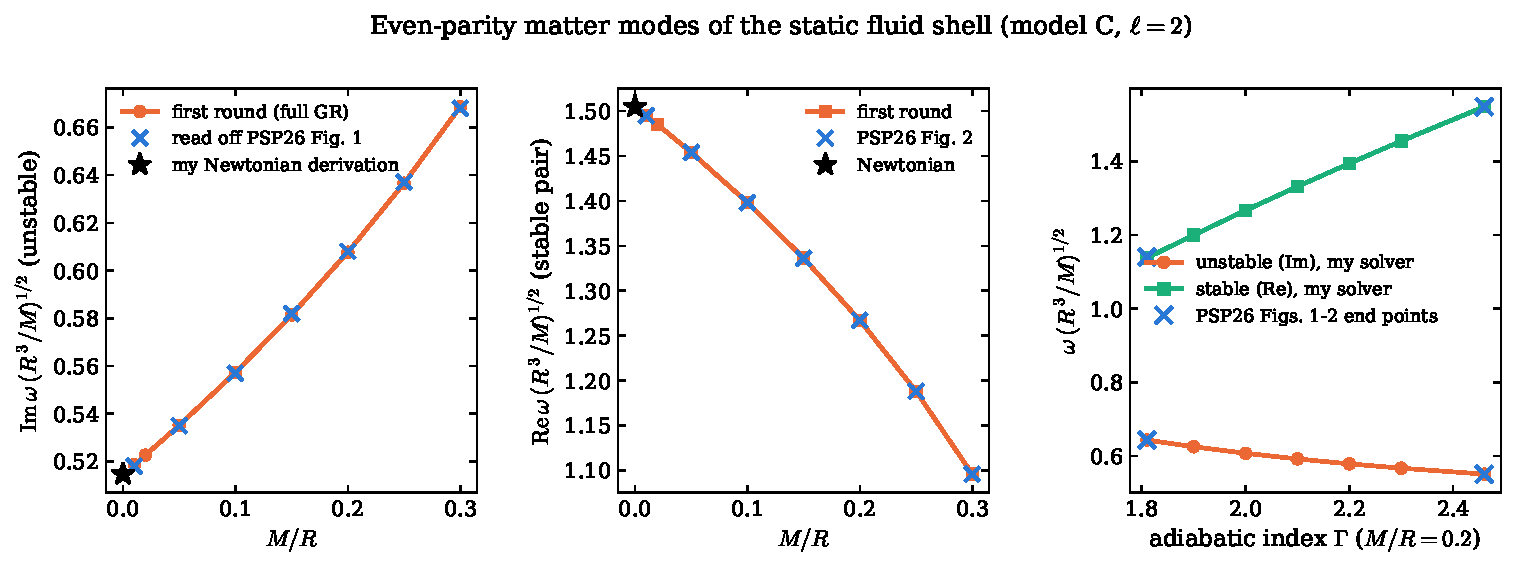
\includegraphics[width=\textwidth]{r2_fig2_matter_modes.pdf}
\caption{Matter modes of the static fluid shell: first round, values read off PSP26, our Newtonian limit and our
$\Gamma$ scan.}\label{fig:matter}
\end{figure}

%=====================================================================================================
\section{Model A: the frozen domain wall}\label{sec:A}
\paragraph{What is confirmed.} The overdetermination (8 equations, 6 unknowns, rank 6 vs 8) is in the first-round
log. With the first round's prescription (all four metric-continuity rows plus the trace and trace-free angular
Israel rows) the relative constraint violation falls as $\omega^{-1}$ and $|\mathcal R+\mathcal T-1|$ as $\omega^{-2}$
(local exponents $-2.00$ between $\omega M=2$ and $32$; A2 \OK). The kinematic statement $\dddot T_0\propto\ddot R^2$
follows from $\dot T_0=\beta/f$, $\partial\dot T_0/\partial\dot R=\dot R/f\beta$ (A3 \OK).

\paragraph{What fails (A4, A5 \NO).} The first round's justification of its prescription is that the $\tau\tau$
and $\tau A$ rows are ``constraints'' which an exact solution would satisfy automatically. For the frozen ansatz,
which is not a solution, every choice of two Israel rows is equally an approximation. We kept the metric-continuity
rows (the first junction condition must hold) and tried all six choices (\file{c06d}, \file{c06e},
Fig.~\ref{fig:modelA}):
\begin{center}\small
\resizebox{\textwidth}{!}{\begin{tabular}{lcccc}\toprule
imposed Israel rows & $\mathcal R(\omega M=30)$, $R=3M$ & $|\mathcal R+\mathcal T-1|$ & residual of dropped rows & lowest QNM, $R=6M$\\\midrule
trace + trace-free (first round) & $6.8\times10^{-5}$ & $1.7\times10^{-4}$ & $1.9\times10^{-4}$ & $0.18120-0.22393i$\\
$\tau\tau$ + trace-free & $1.8\times10^{-6}$ & $10^{-13}$ & $0.26$ & $0.13978-0.27050i$\\
$\tau A$ + trace-free & $3.4\times10^{-6}$ & $5.6\times10^{-5}$ & $0.13$ & $0.17063-0.26403i$\\
$\tau\tau$ + trace & $1.000$ & $3.9\times10^{-9}$ & $2.1\times10^{-5}$ & (none near)\\
$\tau A$ + trace & $0.9998$ & $2.8\times10^{-8}$ & $2.1\times10^{-5}$ & (not computed)\\
$\tau\tau+\tau A$ & $0.9999$ & $10^{-13}$ & $6.7\times10^{-5}$ & $0.16818-0.19045i$\\\bottomrule
\end{tabular}}\end{center}
(For comparison: odd parity and model C give $1.8\times10^{-6}$ and fundamental modes $0.24739-0.22534i$ and
$0.13710-0.26885i$.) The predictions differ at $O(1)$, and the differences do not shrink with $\omega$. Three
observations settle the matter:
(i) with the first round's choice the energy error exceeds $\mathcal R$ itself at every high frequency
($3.8\times10^{-2}$ vs $1.6\times10^{-2}$ at $\omega M=2$; $1.5\times10^{-4}$ vs $6.0\times10^{-5}$ at $\omega M=32$, $R=3M$):
the quoted $\mathcal R$ of model A has no significant digit;
(ii) choices that satisfy the dropped rows better (e.g.\ $\tau\tau$+trace, residual $2\times10^{-5}$) predict total
reflection instead;
(iii) the choice $\tau\tau$+trace-free conserves energy exactly and reproduces the universal high-frequency law
$\mathcal R\simeq\Delta^2_{\rm odd}/4\omega^2$ shared by odd parity and model C.
Consequently the statements ``Model A \dots\ reflects much more strongly, and its $\mathcal R$ decays more slowly''
(derivation Sec.~6.2 item 5, Figs.~2, 11) and ``its even-parity results should be read as
$O(\omega_{\rm dyn}/\omega)$-accurate'' are not supported. Together with Sec.~\ref{sec:bg} (B12) -- the wall's QNMs
have $|\omega|\approx2$--$5\,\omega_{\rm dyn}$ -- the even-parity model-A spectrum and reflectivity should be regarded as
undetermined by the frozen approximation. The odd sector of model A is unaffected (exactly consistent, O5).

\begin{figure}[t]\centering
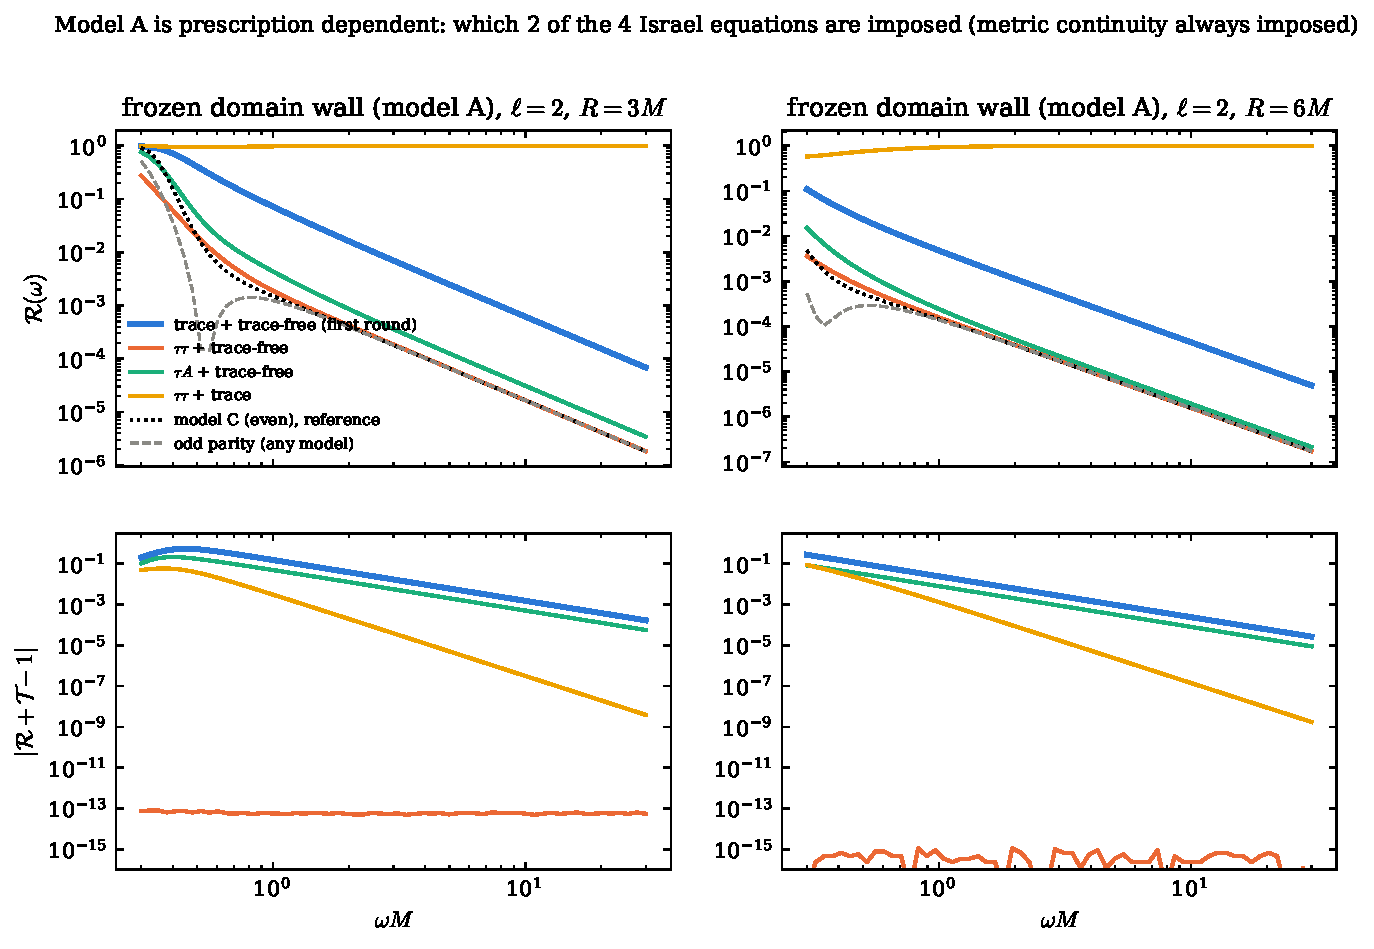
\includegraphics[width=\textwidth]{r2_fig3_modelA_prescriptions.pdf}
\caption{Reflectivity and energy balance of the frozen domain wall for four admissible prescriptions (metric
continuity always imposed). The first-round prescription (thick blue) is not singled out by any criterion.}\label{fig:modelA}
\end{figure}

%=====================================================================================================
\section{Numerical methods and results}\label{sec:num}
\paragraph{Exterior machinery.} The continued-fraction coefficients reproduce Pani et al.\ (B4)/(B7) under
$\omega\to-\omega$ (their time dependence is $e^{+i\omega t}$; we compared the printed $c_i,d_i,e_i$). Their
convergence condition ($R_2/2<a<R_2$, ``$R_2>2$'' in units $2M=1$) is equivalent to the first round's $R_2\ge4M$
(N1 \OK). The asymptotic recursion (5.5) was re-derived symbolically for $k=1\dots5$ (N2 \OK).

\paragraph{Scattering coefficients} (\file{c04}). Our solver recomputed $\mathcal R$ and $\mathcal T$ at 12 frequencies of
nine configurations (odd $\ell=2,3$; even-C $\ell=2,4$; even-A $\ell=2$; $R=2.2$--$6M$). Largest differences from the
first round's Method 1: $1.5\times10^{-11}$ in $\mathcal R$ and $1.3\times10^{-8}$ in $\mathcal T$, the latter set by our own
$|\mathcal R+\mathcal T-1|\sim5\times10^{-9}$. The first round's table gives $\max|\Delta_{12}|=6\times10^{-10}$; the text's
``$\lesssim10^{-10}$'' should read ``$\lesssim10^{-9}$'' (N3 \PART).

\paragraph{QNMs} (\file{c04}). 67 modes (51 catalogue modes -- wave and matter modes of odd, even-C, even-A for
$\ell=2,3$ and $R=2.2$--$10M$ -- and the 16 matter modes of the PSP table) were re-converged with our solver from the first-round values: all wave and growing
modes agree to $10^{-10}$--$10^{-13}$ ($1.6\times10^{-7}$ for the strongly damped $0.78377-0.71437i$ at $R=2.2M$); the
damped imaginary matter modes agree to $10^{-5}$--$10^{-7}$, the same level as the first round's own Method-1/2
difference (N5 \OK). Of the 397 catalogue entries, 28 have $|w_1-w_2|>10^{-8}$ and 8 exceed $10^{-6}$ (max
$6.4\times10^{-5}$); all are below the task's $10^{-4}$, but the claims of $10^{-8}$--$10^{-13}$ are overstated (N4).

\paragraph{Completeness of the catalogue} (N6 \PART).
\begin{itemize}
\item $\ell=2$, even-C: the stable matter pair is absent at $R=2.2,2.5,3M$, although it exists and is continuous with the
tracked mode: $0.185919-0.000030i$ ($2.2M$), $0.212774-0.000206i$ ($2.5M$), $0.197121-0.000310i$ ($3M$). At $R=3M$ the
entry labelled ``matter-stable'' is a duplicate of the unstable mode ($+0.13321i$).
\item $\ell=4$, $R=2.2M$: the unstable matter mode ($0.43726i$) is missing; the entry labelled ``matter-imag-damped''
($1.27806-0.72384i$) is a wave mode.
\end{itemize}
Tables \file{shell_qnm_l2/l4.tex} and \file{qnm_table.csv} inherit these omissions. They do not affect the
physical conclusions (the instability is present for all $\ell$ and $R$ examined).

\paragraph{Other items.} The Boyanov et al.\ estimator is implemented as $|i\omega+\Psi_{,r_*}/\Psi|/|i\omega-\Psi_{,r_*}/\Psi|$,
whose square is compared with $\mathcal R$; the agreement $2$--$4\times10^{-6}$ is consistent with the neglected $O(1/r)$
terms (N7 \OK). In Fig.~5 the estimator's crosses are hidden under the circles. The Method-1 NaN at $\ell=4$,
$\omega M=0.00566$ is present for all three $R=6M$ curves, as stated (N8 \OK).

%=====================================================================================================
\section{Schwarzschild validation, WKB and limits}
\paragraph{QNMs} (\file{c02}). Our 30-digit Leaver solver with $n$-th inversion gives
$\omega M=0.3736716844-0.0889623157i$ for $\ell=2$, $n=0$ and agrees with the first round's twelve values to
$\le1.4\times10^{-16}$, and with the six-digit table of Berti, Cardoso \& Starinets to $\le6\times10^{-7}$ (rounding)
(S1, S2 \OK).

\paragraph{WKB} (S3, S4). The third-order WKB was recomputed from the explicit Iyer--Will formula (1.5a,b)
(coded independently from the hypervirial construction): all twelve values agree with the first round to
$5\times10^{-16}$, which validates the hypervirial code at that order; $\ell=2$, $n=0,1$ give $0.37316-0.08922i$ and
$0.34602-0.27492i$, consistent with the values quoted from Iyer--Will. The sixth-order values could not be compared
with Konoplya's table (full text not accessible); they behave as expected (error $1.4\times10^{-7}$ for $\ell=4,n=0$)
(\NV). The errors quoted in the text for $\ell=2,n=0$ ($7\times10^{-2}$, $1.5\times10^{-3}$, $2.3\times10^{-4}$) are relative
errors $|\Delta\omega|/|\omega|$; the absolute errors are $2.5\times10^{-2}$, $5.7\times10^{-4}$, $8.9\times10^{-5}$.

\paragraph{Black-hole reflectivity} (S5 \OK). With an integrator in $r_*$ (LSODA, start at $r_*=-80M$) we obtain
$\mathcal R=1.548455\times10^{-2}$ at $(2M\omega)^2=1$ and $5.3117\times10^{-9}$ at $(2M\omega)^2=4$, equal to the first
round's values; the scanned Vishveshwara Fig.~2 is consistent (about $1.5\times10^{-2}$ and $\sim10^{-8}$).

\paragraph{Limits} (\file{c08}). Low frequency: $1-\mathcal R\le10^{-15}$ at $\omega M=10^{-3}$ for odd, even-C, even-A
(L1 \OK). High frequency: $\mathcal R/[\Delta^2/(4\omega^2+\Delta^2)]=0.997$--$0.999$ at $\omega M=8$ (L2 \OK). Closed
system: $||S|-1|\le4\times10^{-16}$ (L4 \OK). Black-hole limit (L3 \PART): the approach is real but slow and
oscillatory, the amplitude of the shell contribution scaling like $\Delta_{\rm odd}\propto(R-2M)^{1/2}$; at $\omega M=0.6$,
$\mathcal R/\mathcal R_{\rm BH}=8.4,4.8,3.1,0.32,0.89$ for $R-2M=0.2,0.05,0.01,0.002,0.0002$ (Fig.~\ref{fig:bh}), so the
table value at $2.002M$ (0.00021 vs 0.00066) is not ``consistent'' in the sense of convergence yet. Trapped modes: all
seven values of \file{trapped.tex} reproduced to $\le4\times10^{-12}$; WKB real parts are off by 0.6--6.3\% and imaginary
parts by factors 1.12--2.03 (the text says 1--6\% and $\lesssim2$) (L5 \PART).

\begin{figure}[t]\centering
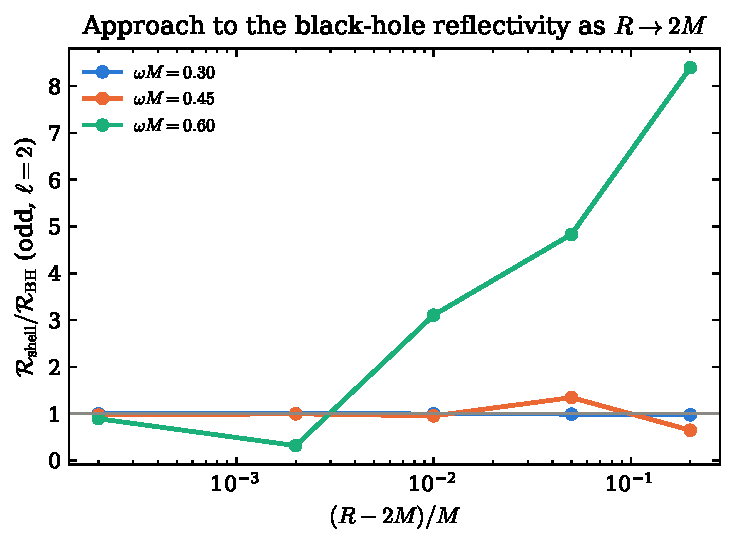
\includegraphics[width=0.55\textwidth]{r2_fig5_bh_limit.pdf}
\caption{Oscillatory approach of the odd-parity shell reflectivity to the black-hole value.}\label{fig:bh}
\end{figure}

%=====================================================================================================
\section{Literature and citations}\label{sec:lit}
\begin{longtable}{p{3.2cm}p{7.6cm}p{4.3cm}}
\caption{Every reference of the first round.}\label{tab:lit}\\\toprule
reference & what the first round uses & status\\\midrule\endhead
Regge--Wheeler 1957 & Eq.~(25) ($k_{\rm eff}^2$, i.e.\ the odd potential), (24), gauge (18), (20) & local PDF (page read); \OK\\
Zerilli 1970 & Eq.~(5), first-order system, Eq.~(3) & local PDF; \OK\\
Vishveshwara 1970 & Fig.~2 & local PDF (scan); \OK\\
Martel--Poisson 2005 & Eqs.~(3.1)--(3.7), (4.1)--(4.3), (4.23)--(4.26), (5.1)--(5.18) & local PDF, all numbers exist; \OK\\
Martel thesis & ``consulted'' & local PDF; not used\\
Ipser--Sikivie 1984 & (2.1)--(2.14), (3.1)--(3.9), quote & local PDF (pages read); \OK\\
Poisson 2004 & (3.49), (3.56), (3.65), (3.68)--(3.70), (3.75)--(3.81) & local PDF, all numbers exist; \OK\\
Abramowitz--Stegun; DLMF 10.50.1 & Riccati--Bessel functions; Wronskian & identity verified numerically; \OK\\
Pani et al.\ 2009 & (3.29), (3.33), (A16), (A20), (A35), App.~B & arXiv v2 PDF; labels and content \OK. Full title has
``I.\ Nonradial oscillations \dots''\\
Pitre--Schneider--Poisson 2026 & (1.1)--(1.2), (2.4)--(2.6), (5.23), (7.8), (7.23)--(7.25), Figs.~1--4 & arXiv PDF;
PRD 113, 124055 (2026). \OK; $\delta p=\Gamma p\,\delta\mu/(\mu+p)$ is PSP26 (2.7)\\
Boyanov et al. & App.~B1, Eqs.~(14), (15), (17), Fig.~1 & arXiv; PRL 135, 151402 (2025) (INSPIRE). \OK\\
Leaver 1985 & continued fraction & INSPIRE; \OK\\
Berti--Cardoso--Starinets 2009 & QNM tables & INSPIRE; values \OK\\
Leins--Nollert--Soffel 1993 & continued fraction about $R_2$ & cited as such by Pani et al.; \OK\\
Schutz--Will 1985; Iyer--Will 1987; Konoplya 2003 & WKB & INSPIRE; order 3 verified; Iyer's companion paper II (PRD 35, 3632) contains
the Schwarzschild tables\\
Hatsuda 2020; Killingbeck 1978 & WKB = Bender--Wu; hypervirial & ADS/APS; \OK\\
Chandrasekhar 1983 & Sec.~4.26, RW$\leftrightarrow$Z map & book not available; map verified; \NV\ (section number)\\
Cardoso--Franzin--Pani 2016 & echoes of ultracompact objects & well known PRL 116, 171101; \OK\\
Yang, Bonga, Pen & eikonal instability & \NO: H.~Yang, B.~Bonga, Z.~Pan, PRL 130, 011402 (2023)\\\bottomrule
\end{longtable}
The honesty statement (PSP26 computed the QNMs of the same system; no published $\mathcal R$, $\mathcal T$ found) is
consistent with our own reading of PSP26 (no reflection coefficients in the parts we read) and a web search.

%=====================================================================================================
\section{Compliance with the task statement}
All required products exist: derivation with the six requested sections; potentials, $\mathcal R/\mathcal T$, method
comparison, complex-plane QNMs, QNMs vs $R/M$, energy-conservation plots; a CSV with the requested columns and a
literature flag. DOP853 with \texttt{rtol}$=10^{-10}$, \texttt{atol}$=10^{-12}$ is used. The requirement that
\emph{every} function carry a docstring citing its equation is only partly met: of 144 functions (including nested
helpers) 57 have no docstring and 59 more cite no source (C5 \PART); the main physics routines are documented. The
first round's corrections to the task statement (Option B does not exist; Option C has no free $\kappa$; interior
frequency $\nu$; the $\sigma\to0$ limit is flat space and the black-hole reflectivity is reached as $R\to2M$ instead)
are all correct.

%=====================================================================================================
\section{Integrity of the first round}\label{sec:integrity}
The SHA-256 hashes of all 102 files of \file{First round} (Python caches excluded) were recorded before the verification
(\file{first_round_sha256_before.txt}) and recomputed at the end (2026-09-25 15:35, \file{first_round_sha256_after.txt}).
The two lists are \textbf{identical}. No file of the first round was created, modified or deleted by the second round;
all executions used copies inside \file{Second round}.


%=====================================================================================================
\section{Recommendations}
\begin{enumerate}
\item Remove or heavily qualify the even-parity model-A results (reflectivity, QNMs, Figs.~2, 6, 11 and the statements
about the wall reflecting more strongly); if kept, show the prescription dependence of Fig.~\ref{fig:modelA}.
\item Correct the time-scale statements of the Discussion (the wall collapses on $\sim R/\sqrt2$).
\item Replace ``$\lesssim10^{-8}$'' / ``$10^{-8}$--$10^{-13}$'' by the actual method agreement ($\le6.4\times10^{-5}$ overall,
$\lesssim10^{-10}$ for wave modes); state that WKB errors are relative.
\item Complete the catalogue (stable matter pairs at $R\le3M$, $\ell=4$ unstable mode at $2.2M$) and fix the labels.
\item Rephrase the Option-B argument (Sec.~\ref{sec:bg}); correct ``U.-L.~Pen'' to ``Z.~Pan''; mention the misprint in
PSP26 (7.6).
\end{enumerate}

\end{document}
